\section{压强在生产和生活中的应用}\label{sec:5-2}

用手压鸡蛋会把鸡蛋压破,脚踩到乒乓球上会把乒乓球踩瘪。
任何物体能够承受的压强都有一定的限度,超过了这个限度,物体就会压坏。
因此,在许多实际问题中,常常要想办法来改变压强的大小。
我们有了压强的知识,就能够根据实际需要来减小或增大压强。

\begin{wrapfigure}[8]{r}{4cm}
    \centering
    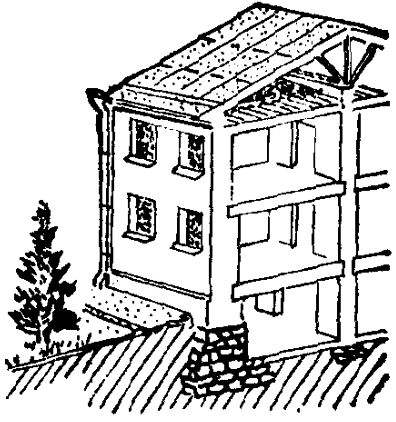
\includegraphics[width=3.5cm]{../pic/czwl1-ch5-4}
    \caption{}\label{fig:5-4}
\end{wrapfigure}

从压强公式可以知道,在压力一定的情况下,受力面积越大,压强就越小。
利用这个知识,在压力不能减小的情况下,我们可以用增大受力面积的方法来减小压强。
在生产和生活中,这样的例子是很多的。

为了防止房屋下沉,需要减小房屋对地基的压强。
把房子的墙基做得比墙厚,就可以增大墙基的底面积,以减小房屋对地基的压强(图 \ref{fig:5-4})。

载重汽车很重,对路面的压力也很大。为了防止压坏路面,就要减小载重汽车对路面的压强。
因此载重汽车的轮胎都做得比小汽车的宽,轮子的个数也较多。
在我国的社会主义建设中,有时需要通过公路把几百吨的大型设备运往工地。
为了解决这类问题,专门制造了有许多轮子的大型平板车,有的大型平板车有 100 多个轮子。

大型拖拉机和坦克自身很重,又经常要在潮湿、松软的土地上行驶,为了防止压坏田地和陷进地里,
需要大大地增加它们跟地面的接触面积。这时只靠增加轮子的个数已经不够了,于是,
人们给大型拖拉机和坦克安装了履带,就象在地上铺了可以随拖拉机和坦克一同移动的钢板一样,
这样就大大地减小了对地面的压强(图 \ref{fig:5-5})。

\begin{wrapfigure}[7]{r}{4cm}
    \centering
    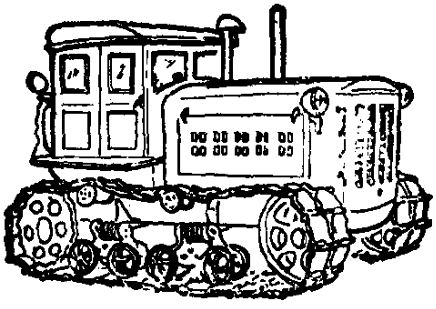
\includegraphics[width=3.5cm]{../pic/czwl1-ch5-5}
    \caption{}\label{fig:5-5}
\end{wrapfigure}

以上讲的都是减小压强的例子。在实际应用中,有时也需要增大压强。
从压强的公式可以知道,在压力一定的情况下,受力面积越小,产生的压强就越大。
因此,在不宜增大压力的情况下,我们可以用减小受力面积的方法来增大压强。
刀子、斧头等的锋刃要磨得很薄,钉子、针、锥子等的尖端要做得很尖,都是为了减小受力面积,
增大压强,使它们在不大的压力下就能够进入物体里去。

我们用手就能把图钉按进木头里,是因为图钉的尖端面积很小,大约只有 $0.05\pfhm$。
用几十牛顿的力按图钉,在图钉尖上就产生几亿帕斯卡的压强。
这个压强大约是履带拖拉机对地面压强的几万倍。

从上面讲的例子可以看出,压强的知识帮助人们解决了许多重要的实际问题。
可见学好物理知识对我们是多么重要。


\lianxi

(1) 书包带宽的比窄的背在身上舒服,为什么?

(2) 砖平放、侧放、竖放在地面上的时候,对地面的压强有什么不同?

(3) 几块完全相同的砖,象图 \ref{fig:5-6} 那样摆在地面上,对地面的压强有什么不同?

\begin{figure}[htbp]
    \centering
    \begin{minipage}{6cm}
    \centering
    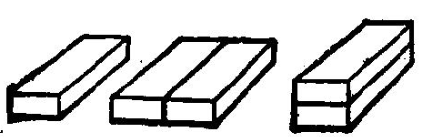
\includegraphics[width=4cm]{../pic/czwl1-ch5-6}
    \caption{}\label{fig:5-6}
    \end{minipage}
    \qquad
    \begin{minipage}{8cm}
    \centering
    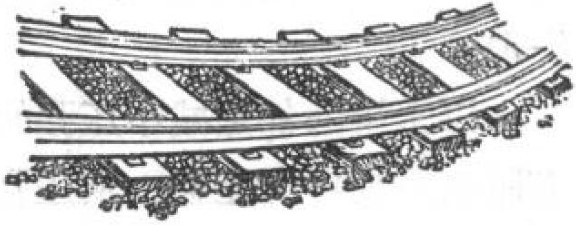
\includegraphics[width=6cm]{../pic/czwl1-ch5-7}
    \caption{}\label{fig:5-7}
    \end{minipage}
\end{figure}

(4) 铁路的钢轨为什么不直接铺在路基上而铺在枕木上(图 \ref{fig:5-7})?

(5) 除了书上的例子以外,自己再举几个生产和生活中增大和减小压强的例子。

(6) 拖拉机的质量是 5150 千克,每条履带跟地面的接触面积约 $0.75 \pfm$,
它对地面的压强是多少?(注意,拖拉机是用两条履带接触地面的)

(7) 上节例题中的人走路时对地面的压强是多少?比较 (6) (7) 两题的结果,你可以得到什么结论?

(8) 封冻的江河冰面能承受的最大压强是 $7 \times 10^4 \pasika$,一辆质量是 20 吨的坦克,
能够在冰面上行驶吗?坦克每条履带跟地面的接触面积是 $2 \pfm$。

(9) 向墙上按图钉,已知图钉帽的面积是 $1 \pflm$,图钉尖的面积是 $0.05 \pfhm$,
手指对图钉帽的压强是 $2\times 10^5 \pasika$,求图钉尖对墙的压强。

(10) 测出物理课本的长和宽,算出它的面积,利用前面测出的课本的质量,算出它受到的重力。
用这些数据,求出课本平放在桌面上时对桌面的压强。

